% !TeX encoding = windows-1250
\chapter{Rezultati}
%\section{Demonstracija metodologije}
Metodologija je demonstrirana na slu�aju usporedbe dvije \gls{pom}-e dobivene s podatcima iz razli�itih izvora i razli�itim postupcima procjene. Duljina razdoblja prikupljanja podataka za obje \gls{pom}-e je $\mathcal{T} = 24 h$, na isti datumu. Za implementaciju demonstracije metodologije kori�teno je programsko okru�enje za statisti�ko ra�unarstvo R.

%\subsubsection{Polazi�no-odredi�na matrica A}
\gls{pom} A je dobivena iz anonimiziranih javno dostupnih  telekomunikacijskih zapisa za grad Shenzhen (\gls{cdr}) \cite{Shenzhen:2017.} postupkom procjene opisanim u radovima \cite{Filjar:2016.} \cite{Filic:2016.} \cite{Desic:2017.}. Rezultat procjene je 8 \gls{pom}-a za vremenske okvire od 3 sata i jedna \gls{pom} za cijeli dan. (Vidi sliku \ref{fig:A})

%\subsubsection{Polazi�no-odredi�na matrica B}
\gls{pom} B je dobivena iz javno dostupnih zapisa polo�aja i statusa (ima putnika/ nema putnika) Taxi vozila u gradu Shenzhenu \cite{Shenzhen:2017.} postupkom procjene opisanim u dodatku \ref{dodatak_taxi}. Rezultat procjene je 8 \gls{pom}-a za vremenske okvire od 3 sata i jedna \gls{pom} za cijeli dan. (Vidi sliku \ref{fig:B})
%\newline
%\newline

\begin{figure}[H]

	\begin{center}	
		\hspace*{-1.6cm}
		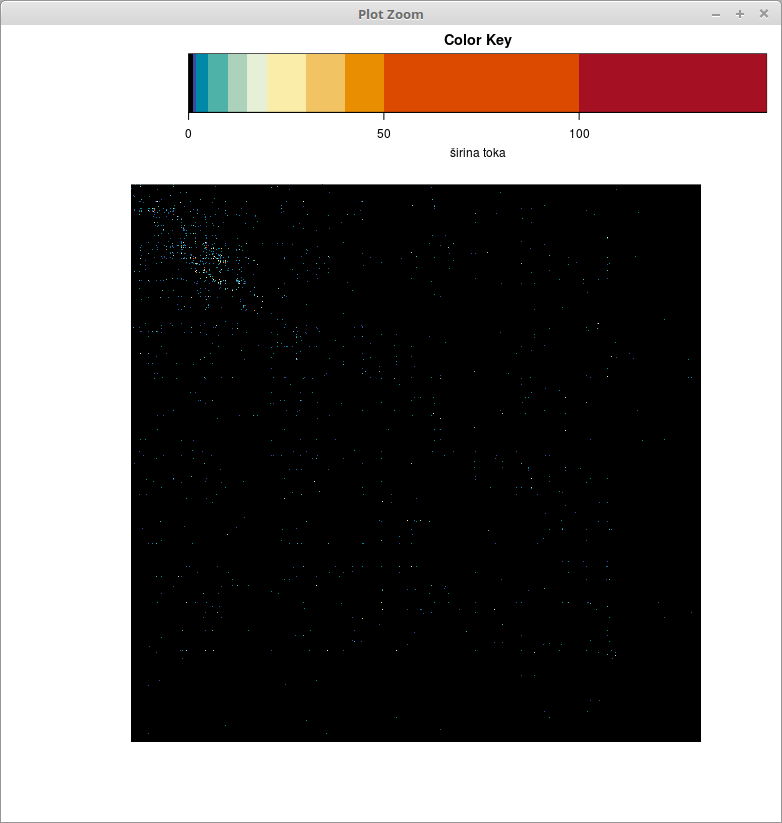
\includegraphics[width=17cm,keepaspectratio=true]{A_0_24_lmat}
		\caption{POM A}
		\label{fig:A}
	\end{center}
\end{figure}

\begin{figure}[H]
	\begin{center}
		\hspace*{-1.6cm}
		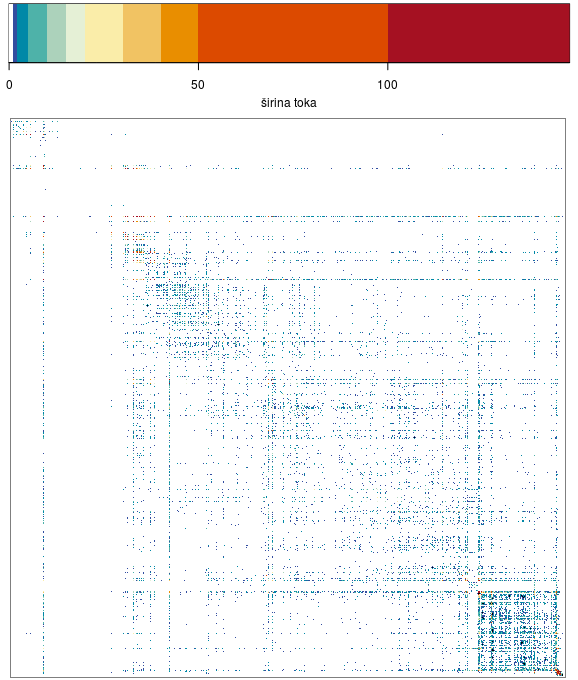
\includegraphics[width=17cm,keepaspectratio=true]{B_0_24_lmat}
		\caption{POM B}
		\label{fig:B}
	\end{center}
\end{figure}


\begin{table}[!htpb]

	\renewcommand{\arraystretch}{1.2}
	\caption{Tablica usporedbe}
	\label{tab:usporedbe}
	\centering
	\hspace*{-1.6cm}
	%\tiny
	\begin{tabular}{|c|c|c|c|c|c|c|c|c|}
		\hline
		POM
		&\makecell{prostorno\\obuhva�anje}
		&\makecell{gusto�a\\informacija}
		&\makecell{prostorna\\zrnatost}&\makecell{vremenska\\zrnatost}
		%&\makecell{Tematska\\Zrnatost}
		%&\makecell{Tematska\\Rezolucija\\Svrhe}
		&\makecell{tematska\\rezolucija\\na�ina kretanja}
		&\makecell{ukupna\\�irina\\toka}
		\\ [0.5ex]
		\hline \hline
		A& {\cellcolor{green!25}}\makecell{neovisno o\\prometnoj\\infrastrukturi}
		&0.008830772
		&$1090\times1090$
		&8
		%&0
		%&0
		&0
		&30878
		\\ [0.5ex]
		\hline
		B
		&\makecell{ \\cesta\\  }
		&\cellcolor{green!25}0.08683223
		&$1090\times1090$
		&8
		%&0
		%&0
		&\cellcolor{green!25}1
		&\cellcolor{green!25}427646
		\\ [0.5ex]
		\hline
		
	\end{tabular}
	
\end{table}

\begin{table}[!htpb]
	\renewcommand{\arraystretch}{1.2}
	
	%\caption{Tablica usporedbe}
	\centering
	\hskip-2.0cm
	%\tiny
	\begin{tabular}{|c|c|c|c|c|c|c|c|c|}
		\hline
		POM
		&\makecell{vremenska\\rezolucija}
		&\makecell{prostorna\\rezolucija}
		\\ [0.5ex]
		\hline \hline
		A
		& *
		& $\approx 75 m $  *
		\\ [0.5ex]
		\hline
		B
		& %\cellcolor{green!25}
		$5 s$
		& %\cellcolor{green!25}
		$\approx 10 m$ (GNSS)
		\\ [0.5ex]
		\hline
		
	\end{tabular}
\\ * vremenska rezolucija je neodre�ena, \\prostorna rezolucija za \gls{cdr} op�enito, prema preporukama \cite{Goulding:2016.}
\end{table}

Prema odnosnim parametrima kvalitete definiranim u sekciji \ref{param} i metodologiji usporedbe definiranoj u poglavlju \ref{met}, \gls{pom} B ukupno ostvaruje bolji rezultat.\\
